\documentclass{article}
\usepackage{amsmath,amssymb}
\usepackage{hyperref}
\usepackage{graphicx}
\usepackage{todonotes}

\title{\bf{Laboratory Project Two: Calibration of an Oriface Meter}}
\author{Jon Langston \& Nicholas Malaya \& Owen O'Neal \\ Department of Mechanical Engineering \\ University of Texas at Austin} \date{}

\begin{document}
\maketitle
\date{}
\newpage
\section{Presentation of Calibration Data}

\textbf{A calibration of the $C_d$ vs $Re$ and comment on whether your
results were as expected.}   

We have adjusted the sample rates down  300 samples at a rate of 100
Hz. The results are shown in Figure 
\ref{oriface-time}, below. The samples appear to still be correlated in
time. 


\begin{figure}[!htb]
  \begin{center}
    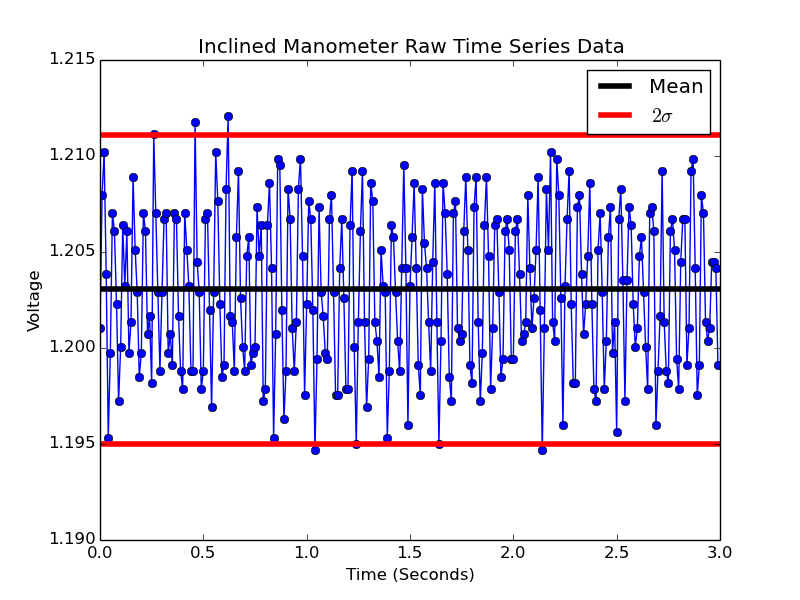
\includegraphics[width = 12 cm]{figs/oriface_time.png}
    \caption{Example raw time series data from a single oriface meter 
      run. The calculated mean of the signal is shown in black, along with
      the two $\sigma$ (standard deviation) confidence interval in
      red.}
    \label{oriface-time}
  \end{center}
\end{figure}

Examining the probability distribution functions in Figure \ref{oriface-hist},
we can see that while the results are clearly better and closer to that
of a gaussian, they are still not normally distributed. 

  \begin{figure}[!htb]
   \begin{center}
    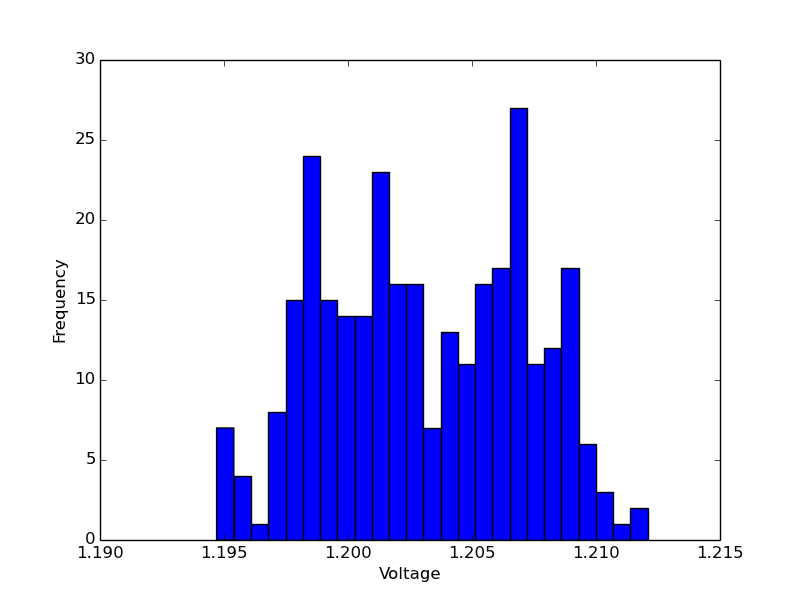
\includegraphics[width = 12 cm]{figs/oriface_hist.png}
    \caption{Histogram depicting the frequency of voltages in our
    signal. This was generated with fifty bins, but the results did not
    appear to be sensitive to the number selected.}
    \label{oriface-hist}
   \end{center}
  \end{figure}

We proceed with our calculations of the quantities of interest. We
intend to plot $C_d$ as a function of Reynolds number. We have not made
a direct measurement of either quantity, and must calculate them as
surrogate quantities from our data. 

The Reynolds number is defined as, 
\begin{equation}
 \text{Re} = \frac{UL}{\nu}.
\end{equation}

The kinematic viscosity ($\nu$) and the pipe diameter ($L$) are
given. We can calculate the bulk fluid velocity ($U$) from our knowledge
of the flow rate and the system dimensions, 
\begin{equation}
 U = \frac{Q}{A} = \frac{Q}{\pi r^2} = \frac{Q}{\pi d^2/4}.
\end{equation}
The Reynolds number is therefore calculated as,
\begin{equation}
 Re = \frac{Q L}{\pi \nu d^2/4}.
\end{equation}

Turning our attention to the calibration coefficient, Equation (9.2)
from page 211 in Stavros' text describes a relation for  
the flow rate as a function of the pressure drop,  
\begin{equation*}
 Q = C_d \frac{\pi d^2 / 4}{\sqrt{1-(d/D)^4}}\sqrt{\frac{2 \Delta p}{\rho}}.
\end{equation*}
This can be manipulated to provide an equation for $C_d$ as, 
\begin{equation}
 C_d = \frac{Q (1-\beta^4)^{1/2}}{\pi d^2/4} \left(\frac{\rho}{2 \Delta
					      P}\right)^{1/2}.
\end{equation}

\newpage
\section{Uncertainty Analysis}

\textbf{Uncertainty of flow rate measured using the orifice meter with
your calibration.} 

\todo{how do we want to approach this?}

\end{document}
